\documentclass[arhiv]{izpit}

\usepackage{graphicx}

\begin{document}

%%%%%%%%%%%%%%%%%%%%%%%%%%%%%%%%%%%%%%%%%%%%%%%%%%%%%%%%%%%%%%%%%%%%%%
%%%%%%%%%%%%%%%%%%%%%%%%%%%%%%%%%%%%%%%%%%%%%%%%%%%%%%%%%%%%%%%%%%%%%%
\izpit[ucilnica=3.10]
  {Programiranje 1: 2.~izpit}
  {16.~marec 2011}
  {Čas reševanja je 120 minut.Vse odgovore utemeljite. Veliko uspeha!}

%%%%%%%%%%%%%%%%%%%%%%%%%%%%%%%%%%%%%%%%%%%%%%%%%%%%%%%%%%%%%%%%%%%%%%
\naloga[\tocke{25}]

\podnaloga
%
Sestavi funkcijo \texttt{najpogostejsi(a)}, ki vrne tisto vrednost v
tabeli \texttt{a}, ki se največkrat ponovi. Če je takih vrednosti več,
naj vrne eno od njih:
%
\begin{verbatim}
>>> najpogostejsi([2,3,4,2,4,2])
2
>>> najpogostejsi([1,1,2,2,1,2])
1
\end{verbatim}

\podnaloga
\textbf{Dodatna naloga (+10 točk):}
%
sestavi še funkcijo \texttt{najpogostejsi\_indeksi}, ki vrne seznam
indeksov, na katerih se pojavi najpogostejša vrednost:
%
\begin{verbatim}
>>> najpogostejsi_indeksi([2,3,3,2,4,2])
[0, 3, 5]
\end{verbatim}


%%%%%%%%%%%%%%%%%%%%%%%%%%%%%%%%%%%%%%%%%%%%%%%%%%%%%%%%%%%%%%%%%%%%%%
\naloga[\tocke{25}]

Dan je razred seznamov \texttt{Seznam}, ki ga lahko naložiš tudi s
spletne učilnice:
%
{\small
\begin{verbatim}
class Seznam():
    def __init__(self):
        self.prazen = True

    def __repr__(self):
        return ("()" if self.prazen else "({0},{1})".format(self.glava, self.rep))

    def dodaj(self, x):
        if self.prazen:
            self.prazen = False
            self.glava = x
            self.rep = Seznam()
        else:
            self.rep.dodaj(x)
        return self

    def dolzina(self):
        return (0 if self.prazen else 1 + self.rep.dolzina())
\end{verbatim}
}

\noindent
Razredu dodaj objektno metodo \texttt{zbrisi(self,k)}, ki iz seznama
\texttt{self} pobriše \texttt{k}-ti element, pri čemer ima prvi
element indeks~$0$. Metoda naj vrne vsebino zbrisanega elementa, ali
\texttt{None}, če seznam nima \texttt{k}-tega elementa:
%
\begin{verbatim}
>>> s = Seznam().dodaj('a').dodaj('b').dodaj('c').dodaj('d')
>>> s
(a,(b,(c,(d,()))))
>>> s.zbrisi(2)
'c'
>>> s
(a,(b,(d,())))
\end{verbatim}

\goodbreak

%%%%%%%%%%%%%%%%%%%%%%%%%%%%%%%%%%%%%%%%%%%%%%%%%%%%%%%%%%%%%%%%%%%%%%
\naloga[\tocke{25}]

Andrej je sestavil funkcijo \texttt{f}:
%
\begin{verbatim}
def f(i,j):
    if j == 0: return 1
    elif i == 0: return 0
    else:
        return f(i-1,j) + i * f(i,j-1)
\end{verbatim}
%
Ko pa je želel izračunati vrednost \texttt{f(42,23)}, je ugotovil, da
funkcija deluje počasi.
%
Sestavi funkcijo \texttt{g}, ki deluje tako kot \texttt{f}, le da je
hitrejša in izračuna \texttt{g(42,23)} v trenutku.

%%%%%%%%%%%%%%%%%%%%%%%%%%%%%%%%%%%%%%%%%%%%%%%%%%%%%%%%%%%%%%%%%%%%%%
\naloga[\tocke{25}]

V Mathematici sestavi funkcijo \texttt{kvadrati[n]}, ki nariše
vgnezdene kvadrate, kot je to prikazano na sliki:
%
\begin{center}
  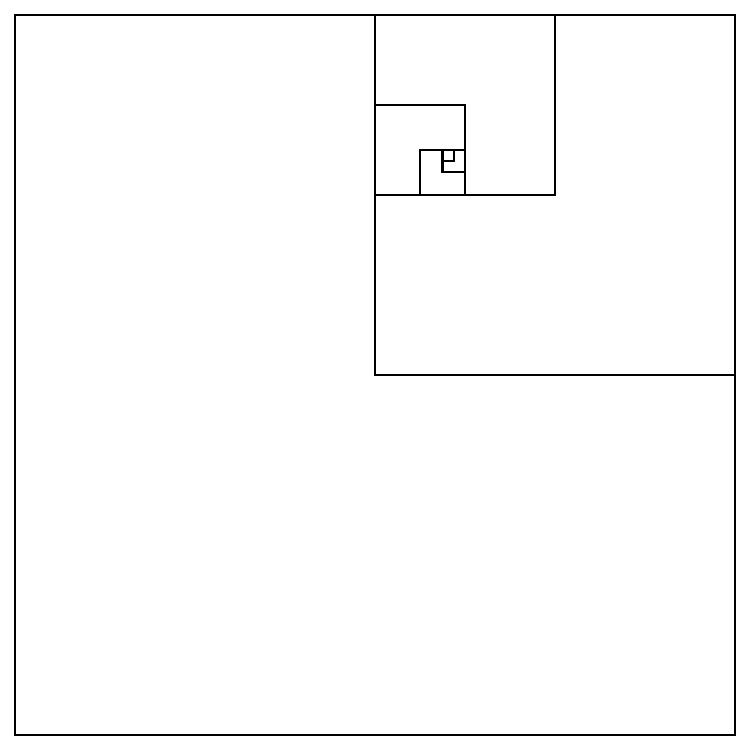
\includegraphics[width=0.4\textwidth]{kvadrati}
\end{center}
%
Vsak naslednji kvadrat je polovico manjši od prejšnjega, število
kvadratov je enako \texttt{n}.


\end{document}

